%!TEX root = DisenoProyecto_LuisGomez.tex
%\begin{consigna}{red} % El bloque "consigna" se usa para poner texto en rojo y dar una pequeña ayuda sobre cómo completar la sección. En cada entrega parcial deben eliminar los comandos begin y end del bloque consigna de las secciones que hayan completado.
%
%El objetivo es que el lector en una o dos páginas entienda de qué trata el proyecto y cuáles son sus desafíos, cuál es la motivación para realizarlo y su importancia.
%
%Se debe introducir el contexto del proyecto, el estado del arte en la temática, describir la propuesta de valor, cúal es el problema que atiende y cuál es la solución que se propone. Se debe dar una descripción funcional de la solución que incluya un diagrama en bloques.
%
%Puede ser útil incluir en esta sección la respuesta a alguna de estas preguntas:
%
%\begin{itemize}
%	\item ¿Cuál es el contexto del proyecto, es un emprendimiento personal, un proyecto para una empresa, es parte del programa de vinculación con empresas del posgrado?
%	\item ¿Existen o aplican condiciones especiales al proyecto, financiamiento de algún programa público o privado, acuerdos de confidencialidad, acuerdos sobre la propiedad intelectual de los entregables u otros?
%	\item ¿Cómo se compara la solución propuesta con el estado del arte en el campo de aplicación? ¿En qué aspectos destaca?
%	\item ¿Ayuda a la explicación si se incluye un lienzo Canvas del Modelo de Negocio?
%	\item ¿En qué estado del ciclo de vida está la solución que se propone?
%	\item ¿Cuáles son las características del cliente (el adoptante de los entregables del proyecto) qué valora, qué necesita?
%	\item ¿Por dónde pasa la innovación?
%\end{itemize}
%
%La descripción técnica-conceptual \textbf{debe incluir al menos un diagrama en bloques del sistema} y descripción funcional de la solución propuesta.
%
%Las figuras se deben mencionar en el texto ANTES de que aparezcan con una frase como la siguiente: ``En la Figura \ref{fig:diagBloques} se presenta el diagrama en bloques del sistema. Se observa que...''.  La regla es que las figuras nunca pueden ir antes de ser mencionadas en el texto, porque sino el lector no entiende por qué de pronto aparece una figura.
%\item ¿Por dónde pasa la innovación?
%\item ¿Cuáles son las características del cliente (el adoptante de los entregables del proyecto) qué valora, qué necesita?

%¿En qué estado del ciclo de vida está la solución que se propone?

En el contexto actual de gestión ambiental de las grandes ciudades, los instrumentos para medir el material particulado fino (MP2,5) se han convertido en herramientas esenciales. La creciente contaminación atmosférica se cuenta entre las principales causas de muertes prematuras en el mundo, de manera directa e indirecta. Sin embargo, lograr una medición precisa del MP2,5 representa un desafío significativo debido a los elevados costos y los complejos requisitos técnicos involucrados. En muchas áreas urbanas, especialmente en las menos desarrolladas, persiste la incertidumbre acerca de los niveles de exposición al MP2,5 a los que está sometida la población. En respuesta a este desafío, la presente propuesta de proyecto busca diseñar un instrumento para la medición del MP2,5 que, utilizando sensores de bajo costo, aspire a acercarse a los estándares de los equipos analíticos de alto rendimiento que se emplean actualmente, pero a un precio notablemente reducido. Este proyecto está íntimamente ligado a la trayectoria y formación profesional del autor del presente trabajo, como químico atmosférico especializado en la calidad del aire urbano.

Con base en lo anteriormente expuesto, el objetivo de este proyecto es desarrollar un instrumento especializado en la medición del material particulado fino atmosférico urbano (MP2,5). Este instrumento no solo será capaz de almacenar y transmitir los datos recopilados, sino que también se espera superar la precisión que ofrecen los sensores de bajo costo actualmente en el mercado. Como innovación, se propone emplear un conjunto de tres sensores de MP2,5 en un mismo instrumento, coordinados por un microprocesador. Este último será encargado de realizar los cálculos, coordinar el almacenamiento y transmisión de los datos (ver figura \ref{fig:diagBloques}). Al utilizar tres sensores ópticos de MP2,5 operando en simultáneo, se prevé la obtención de mediciones replicadas, lo que permitirá ejecutar análisis estadísticos en tiempo real. Esto facilitará la obtención de promedios y la validación o descarte de datos atípicos. Se hipotetiza que esta estrategia mejorará tanto la precisión como la exactitud de las mediciones y, además, añadirá robustez al sistema. Es decir, si un sensor llegara a fallar, el mal funcionamiento podría detectarse rápidamente, mitigando el riesgo de una interrupción completa del sistema.

Dada la creciente preocupación pública sobre la contaminación atmosférica urbana, tanto desde la perspectiva ambiental como de salud, es probable que autoridades a nivel municipal y gubernamental encuentren este tipo de sistemas de monitoreo altamente relevantes. Estos instrumentos, siendo más asequibles que las tecnologías de monitoreo tradicionales, facilitarían una mayor cobertura en áreas que actualmente carecen de mediciones. Este incremento en la cobertura permitiría evaluar la exposición humana al MP2,5 y podría aportar datos cruciales para monitorear la efectividad de políticas públicas, como los planes de descontaminación atmosférica implementados en diversas ciudades. Adicionalmente, estos sistemas pueden ayudar, como parte del fundamento, a la puesta en marcha de medidas preventivas y correctivas en relación con las emisiones y las concentraciones de MP2,5. 

Dentro del contexto de las soluciones para el monitoreo ambiental, estos dispositivos podrían ser una alternativa coste-efectiva para la gestión de la calidad del aire en entornos urbanos. Su asequibilidad económica, en comparación con los sistemas de monitoreo tradicionales, unida a una mayor precisión y robustez, podría ser valorada positivamente por entidades públicas. Se estima que su implementación facilitaría la gestión de la calidad del aire, sin generar una carga financiera excesiva en los recursos públicos.



\subsection{Destalles del equipo, la tecnología del sensor y muestreo estadístico}

En la figura \ref{fig:diagBloques}, se presenta el diagrama en bloques del instrumento. En él, se puede apreciar un microcontrolador central responsable de gestionar: tres sensores de MP2,5, encargados de medir el contaminante; un sistema de almacenamiento de datos local y un sistema encargado de la transmisión de los registros hacia un servidor remoto. Además, incluye un reloj de tiempo real (RTC) que registra el momento de cada medición y un sistema de alimentación, compatible con la red eléctrica.


\begin{figure}[htpb]
	\centering
	\shorthandoff{<>} % Desactivar caracteres problemáticos
	\begin{tikzpicture}[ node distance=1cm]
	% Nodes
	\node (microcontroller) 
	[draw, rectangle, fill=blue!10!white, align=center] 						
	{\textbf{Microcontrolador}\\ \rotatebox{90}{\faMicrochip}};  
	
	\node (sensor1) 		
	[above right=of microcontroller, draw, rectangle, fill=red!10!white, align=center, yshift=0.2cm, xshift=0.3cm] 	
	{Sensor de\\MP2,5 \faSmog};
	
	\node (sensor2) 		
	[right=of microcontroller, draw, rectangle, fill=red!10!white, align=center] 		
	{Sensor de\\MP2,5 \faSmog};
	
	\node (sensor3) 		
	[below right=of microcontroller, draw, rectangle, fill=red!10!white, align=center, , yshift=-0.2cm, xshift=0.3cm] 	
	{Sensor de\\MP2,5 \faSmog};
	
	\node (storage) 		
	[below=of microcontroller, draw, fill=yellow!10!white, rectangle, align=center] 		
	{Sistema de \\ almacenamiento  \faSdCard }; % \faDatabase
	
	\node (transmission) 	
	[above=of microcontroller, draw, rectangle, align=center] 		
	{Sistema de transmi-\\sión de datos  \faSignal};
	
	\node (rtc) 			
	[above left=of microcontroller, draw, rectangle, align=center, yshift=-1.5cm, xshift=-.33cm]  
	{RTC \faClock[regular]};
	
	\node (power) 			
	[below left=of microcontroller, draw, rectangle, align=center,yshift=-0.2cm, xshift=0.0cm] 	
	{Fuente de\\poder \faBatteryQuarter};
	
	\node (cabinet) 		[above right=of transmission,  xshift=-6.8cm,yshift=-0.7cm]     {\textbf{Gabinete} \faCloudSunRain};
	
	% Bounding Box
	\begin{scope}[on background layer]
	\node[fill=gray!10,  draw, rectangle, rounded corners, fit=(cabinet) (sensor2) (rtc) (storage) (transmission)] {};
	\end{scope}
	
	% Arrows
	\draw[<->] (microcontroller) -- (sensor1);
	\draw[<->] (microcontroller) -- (sensor2);
	\draw[<->] (microcontroller) -- (sensor3);
	\draw[<->] (microcontroller) -- (storage);
	\draw[<->] (microcontroller) -- (transmission);
	\draw[->] (rtc) -- (microcontroller);
	\draw[->] (power) -- (microcontroller);
	\end{tikzpicture}
	\shorthandon{<>} % Reactivar caracteres problemáticos
	\caption{Esquema de bloques del instrumento.}
	\label{fig:diagBloques}
\end{figure}
	





El funcionamiento de los sensores escogidos para esta investigación se fundamenta en el fenómeno de la difracción de luz láser. Concretamente, cuando una partícula en suspensión intercepta un haz láser, se produce una dispersión angular de la luz, la cual es proporcional al tamaño de la partícula involucrada. El patrón de dispersión óptica resultante se captura mediante un detector. Este enfoque presenta algunas mejoras sobre los métodos gravimétricos convencionales, al ofrecer ventajas como la reducción de costos y un incremento notable en la velocidad de muestreo. Sin embargo, es imperativo reconocer ciertas limitaciones inherentes a esta tecnología, tales como una menor precisión y exactitud en comparación con técnicas estándar. Cabe señalar que los instrumentos ópticos todavía no han obtenido la certificación de la Agencia de Protección Ambiental (EPA) como métodos analíticos estándar para la cuantificación de partículas finas en el aire.

Para evaluar cómo el número de muestras (\( n \)) afecta la precisión y la exactitud de un sensor de material particulado fino, se deben considerar las métricas como media, varianza y desviación estándar de la muestra. De acuerdo a esto, la precisión se relaciona con la dispersión de las mediciones y se puede estimar mediante la desviación estándar muestral ($s$). A medida que \( n \) aumenta, el error estándar de la media (\( \text{SEM} \)) disminuye, lo cual se puede expresar como:

\[
\text{SEM} = \frac{s}{\sqrt{n}}
\]

Por lo tanto, un incremento en \( n \) resultará en una disminución de \( \text{SEM} \), mejorando así la precisión del instrumento.

Para evaluar la exactitud, podemos usar el valor medio muestral (\( \bar{x} \)) y compararlo con un valor de referencia conocido (\( \mu \)). La diferencia absoluta entre \( \bar{x} \) y \( \mu \) proporciona una medida de la exactitud del instrumento. Dado que \( \bar{x} \) es un estimador insesgado de \( \mu \), su exactitud mejora con un mayor número de muestras, acercándose más al valor verdadero \( \mu \) debido al Teorema del Límite Central.


%\begin{figure}[htpb]
%	\centering
%	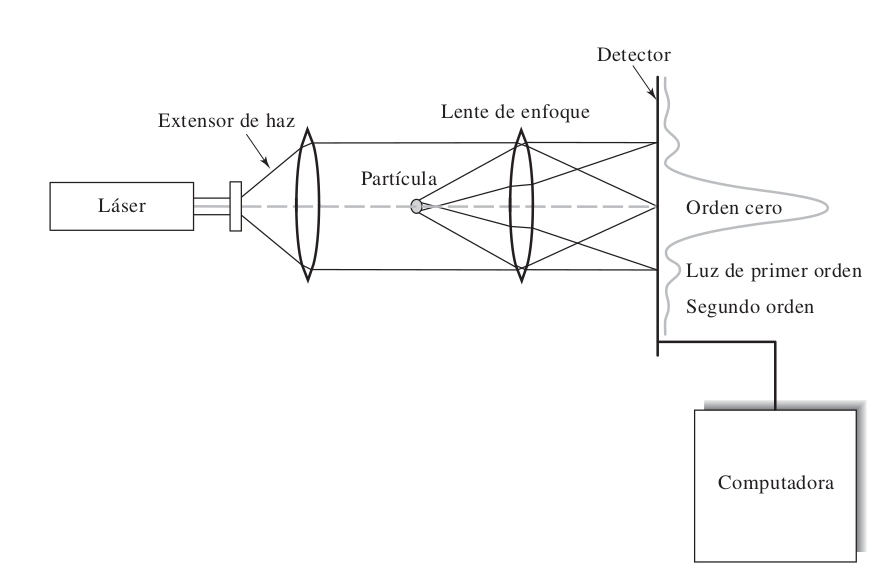
\includegraphics[width=0.65\linewidth]{Figuras/difracion_laser}
%	\caption{Esquema de un sensor de difracción láser típico, empleado para la medición de material particulado fino (fuente:Scookg 2021)}
%	\label{fig:difracionlaser}
%\end{figure}



